\graphicspath{{chapters/5_experimentos/figures/}}

\chapter{Experimentación}\label{chap:experiments}

Para analizar el rendimiento de la implementación, se realizaron experimentos en distintas tarjetas gráficas.
La escena utilizada se muestra en la figura \ref{fig:cornell-box-full}.
Esta escena presenta luz indirecta difusa, luz indirecta especular y sombras suaves.

\begin{figure}
	\centering
	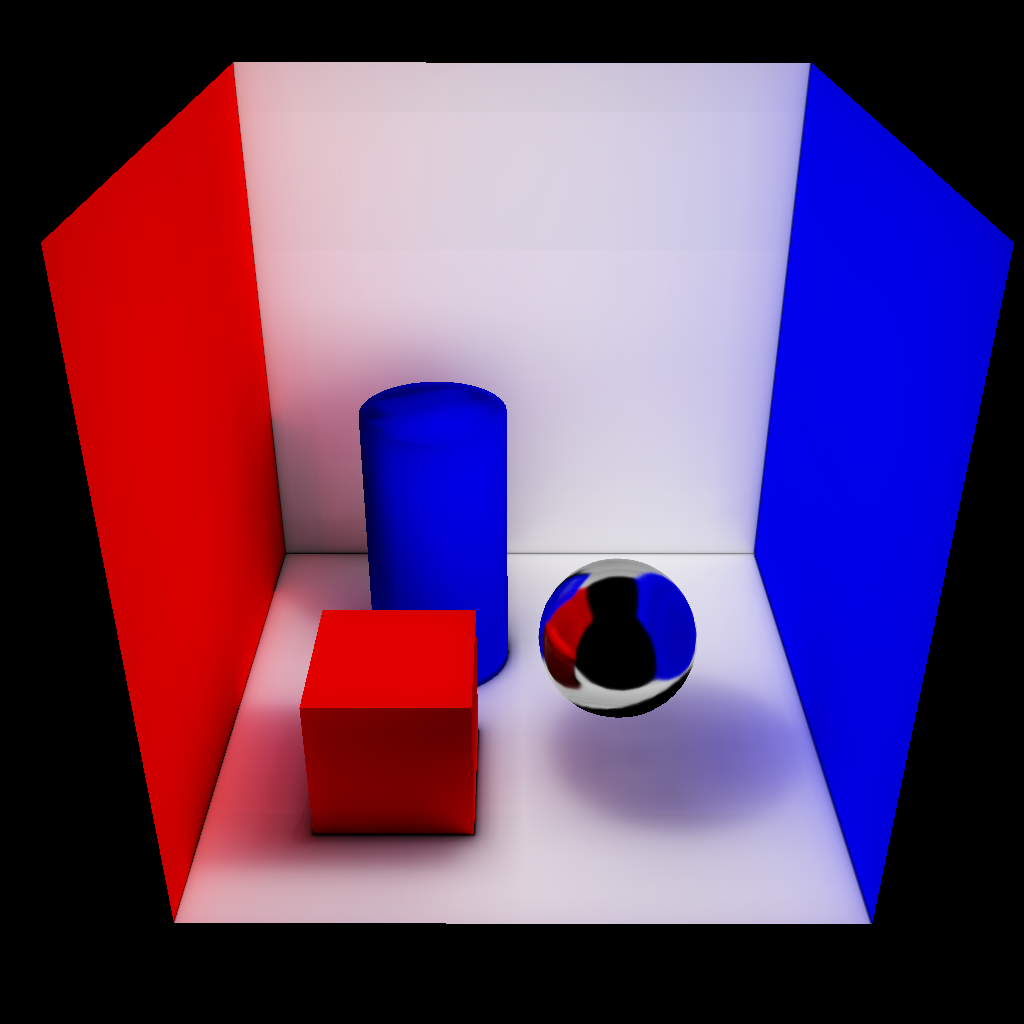
\includegraphics[width=\textwidth]{cornell-box-full.png}
	\caption{Escena con iluminación indirecta mediante \textit{voxel cone tracing}}
	\label{fig:cornell-box-full}
\end{figure}

Los experimentos varian la cantidad de vóxeles por dimensión, y registran los cuadros por segundo alcanzados (FPS) y el tiempo de construcción del \textit{octree} en segundos.
Para conseguir los FPS se corrió el programa por un minuto, tomando una muestra de este valor cada segundo, luego se promediaron.
Para el tiempo de construcción del \textit{octree}, se construyó 50 veces y se promedió el tiempo.
Para que el cache no afectara estas ejecuciones en serie, se realizaron en procesos separados.

En las tablas \ref{tab:cisco-laptop}, \ref{tab:pizzo-laptop} y \ref{tab:pizzo-desktop} se muestran los resultados de estos experimentos en tarjetas Intel Mesa ADL GT2, ??? y Nvidia RTX 4070 respectivamente.
Una observacion es que la implementación parece no estar bien optimizada, dado que en las tarjetas gráficas de laptops en las que se ejecutó, se consiguieron muy pocos cuadros por segundo y tiempos muy lentos de construcción del octree.
Los valores de estas métricas son mucho menores que en las del artículo original del algoritmo, en el que se mostraron entre 20 y 30 cuadros por segundo y 280 milisegundos de construcción del \textit{octree}, en lugar de segundos.

Otra observación es que la tarjeta Nvidia RTX 4070 trae excelentes resultados en terminos de cuadros por segundo, pero sorprendentemente es más lenta que la Intel Mesa ADL GT2 en construír el \textit{octree}.
Esto puede deberse a que la primer tarjeta posee mucho más paralelización, por lo que puede realizar todos los trazados de conos sin problemas, pero este no es el cuello de botella para la construcción del \textit{octree}.
En la construcción, probablemente lo que más este beneficiando a la segunda tarjeta es la cercanía física entre CPU y GPU, que implica una comunicación más rápida.

\begin{table}
\centering
\begin{tabular}{|c|c|c|}
	\hline
	\textbf{Vóxeles} & \textbf{FPS} & \textbf{Construcción del \textit{octree}} \\
	\hline
	$256$ & $14.470$ & $1.451$ \\
	\hline
	$512$ & $11.301$ & $1.490$ \\
	\hline
	$1024$ & $9.215$ & $1.656$ \\
	\hline
\end{tabular}
\caption{Experimentos para una Intel Mesa ADL GT2}
\label{tab:cisco-laptop}
\end{table}

\begin{table}
\centering
\begin{tabular}{|c|c|c|}
	\hline
	\textbf{Vóxeles} & \textbf{FPS} & \textbf{Construcción del \textit{octree}} \\
	\hline
	$256$ & $12.632$ & $2.461$ \\
	\hline
	$512$ & $10.363$ & $2.780$ \\
	\hline
	$1024$ & $8.825$ & $3.245$ \\
	\hline
\end{tabular}
\caption{Experimentos para una ???}
\label{tab:pizzo-laptop}
\end{table}

\begin{table}
\centering
\begin{tabular}{|c|c|c|}
	\hline
	\textbf{Vóxeles} & \textbf{FPS} & \textbf{Construcción del \textit{octree}} \\
	\hline
	$256$ & $141.570$ & $1.949$ \\
	\hline
	$512$ & $141.496$ & $1.936$ \\
	\hline
	$1024$ & $141.406$ & $1.950$ \\
	\hline
\end{tabular}
\caption{Experimentos para una RTX 4070}
\label{tab:pizzo-desktop}
\end{table}
